\documentclass[9pt,twocolumn,twoside]{pnas-new}
% Use the lineno option to display guide line numbers if required.

\templatetype{pnasresearcharticle} % Choose template
% {pnasresearcharticle} = Template for a two-column research article
% {pnasmathematics} %= Template for a one-column mathematics article
% {pnasinvited} %= Template for a PNAS invited submission

\newcommand{\ud}{\text{d}}

\begin{document}


\title{Competitive (eco-evolutionary?) mechanism locking body~size after population collapse} % Suggestions?
% Eco-evolutionary trait changes hinders recovery after population collaps 


% Use letters for affiliations, numbers to show equal authorship (if applicable) and to indicate the corresponding author
\author[a]{Mikael Ohlsson}
\author[a]{György Barabás}
\author[b]{Max Lindmark}
\author[b,c]{Michele Casini}
\author[b]{Valerio Bartolino}
\author[b]{Mattias Sköld}
\author[a]{Anna Eklöf}

\affil[a]{Biology, Linköping University, Department of Physics, Chemistry and Biology, Linköping University, 581 83 Linköping, Sweden}
\affil[b]{Department of Aquatic Resources, Institute of Marine Research, Swedish University of Agricultural Sciences, Institute of Marine Research, Turistgatan 5, 453 30 Lysekil, Sweden}
\affil[c]{Department of Biological, Geological and Environmental Sciences, University of Bologna, Via Selmi 3, 40126 Bologna, Italy}

% Please give the surname of the lead author for the running footer
\leadauthor{Ohlsson}

% Please add a significance statement to explain the relevance of your work
\significancestatement{Authors must submit a 120-word maximum statement about the significance of their research paper written at a level understandable to an undergraduate educated scientist outside their field of speciality. The primary goal of the significance statement is to explain the relevance of the work in broad context to a broad readership. The significance statement appears in the paper itself and is required for all research papers.}

% Please include corresponding author, author contribution and author declaration information
\authorcontributions{M.O., G.B., and A.E. designed the study. M.O. and G.B. wrote the code for the eco-evolutionary model. M.L. and M.C. constructed the model for predicting biomass densities. M.O. performed the simulations and analyses. M.O., G.B., and A.E. wrote the paper. All authors made significant contributions to the final version of the manuscript.}
\authordeclaration{The authors declare no competing interests.}
%\equalauthors{\textsuperscript{1}A.O.(Author One) contributed equally to this work with A.T. (Author Two) (remove if not applicable).}
\correspondingauthor{\textsuperscript{1}To whom correspondence may be addressed. E-mail: mikael.ohlsson@liu.se}

% At least three keywords are required at submission. Please provide three to five keywords, separated by the pipe symbol.

\keywords{alternative stable states $|$ body size $|$ eco-evolutionary dynamics $|$ population collapse $|$ population recovery}

\begin{abstract}  
%Intense harvest and environmental changes can cause species populations to collapse, often without a positive trend after alleviating the stressors. While traditional approaches can partially explain a slow recovery, they fail to predict the observed lack of recovery. The stressors are often accompanied by considerable selection pressure. For example, fishing generally targets larger individuals, causing a selection pressure towards smaller individuals. A neglected aspect related to the change in body size is how it can influence competitive relationships with other species. This is exemplified by the Atlantic cod (\textit{Gadus morhua}) population in the Baltic Sea, where the cod population has collapsed to both small population numbers and small body sizes after decades of intense fishing and environmental changes. Cod's lack of recovery after stopping fishing suggests additional factors need consideration. Here, we present an eco-evolutionary model, which accounts for the development of body size while influenced by fishing, environmental effects and competitive dynamics with dietarily similar species. Our model shows how, for cod in the Baltic Sea, the shift to smaller cod body size has swapped the altered its diet, and thus its competitive relationship with dietarily related flounder species, with flounder now locking cod into its smaller body size. Spatial data from the Baltic Sea align with the model: regions with more flounder have cod with smaller sizes and more dissimilar diets. We conclude that simply reducing fishing pressure may be insufficient for recovery; restoration efforts must also consider the cod's altered ecological role.
Intense harvest and environmental changes can cause species populations to collapse, and lack of recovey even after alleviating the stressors are quite common. Stressors are often accompanied by considerable selection pressure, for example fishing, which generally targets larger individuals. Subsequent trait changes can influence the involved species' ecological roles, potentially causing the observed lack of recovery. Here, using an eco-evolutionary model, we show how the change in body size can lead to altered diet and interspecific competition, with the new competitive relationship locking a species into an altered state. The competitor keeps the affected species from its previous diet, hindering recovery from the population collapse. This applies even after removing other selective pressures, providing a possible factor for why some populations do not recover even after alleviating direct causes. We relate this mechanism to the collapsed population of Atlantic Cod (\textit{Gadus morhua}) in the Baltic Sea, which has decreased in both population size and body size from decades of intense fishing and environmental change. Our model shows how the current situation, of ceased fishing but no observed recovery, may be explained by a new competitive relationship with the dietarily related flounder species locking the cod population into its smaller state. Spatial data from the Baltic Sea align with the model: regions with more flounder have cod with smaller sizes and more dissimilar diets. We conclude that simply reducing harvesting pressure are insufficient for recovery; restoration efforts must also consider altered species interactions and their changed ecological roles.
\end{abstract}


\dates{This manuscript was compiled on \today}
\doi{\url{www.pnas.org/cgi/doi/10.1073/pnas.XXXXXXXXXX}}


\maketitle
\thispagestyle{firststyle}
\ifthenelse{\boolean{shortarticle}}{\ifthenelse{\boolean{singlecolumn}}{\abscontentformatted}{\abscontent}}{}

\firstpage[4]{4}

Decades of environmental change and anthropogenic pressures have led to the urgent situation of population collapses of many marine fish species \cite{Hutchings2004, Neubauer2013}. While some populations can recover from well-managed fisheries \citep{Hilborn2009, Duarte2020}, the situation of other populations is sometimes more complex with continuous declines despite the cessation of fishing \citep{Kuparinen2014, Neuenhoff2019}. Slow or absent recovery is common for such populations and is typically attributed to Allee effects, where lower population size interferes with the recovery \citep{Kuparinen2014}. Such explanations are however generally only partially sufficient for the lack of recovery, as with time, the populations are expected to recover after fishing stops unless further factors interact \citep{Neuenhoff2019}. 

Another factor impacting this dynamic is body size dependence \citep{Ahti2020}. Fishing is widely recognized to exert selective pressure on fish populations \citep{Law2000, Kuparinen2009}, with fisheries generally targeting larger individuals \citep{Kuparinen2009, Hunter2015}. Body size is heritable, so intense fishing of larger individuals will create an evolutionary advantage for smaller individuals \citep{Nielsen2014, Kuparinen2017}. As the body size of a species is modified, the species' interspecific interactions can also change, which may further influence the body size \citep{Edeline2021}. While size dependence is recognized to influence dietary preferences directly \citep{Ahti2020}, this aspect may be further influenced by changes to interspecific competitive relationships \citep{Edeline2021}.

The Baltic Sea is a semi-enclosed basin where the cod population (\textit{Gadus morhua}) has collapsed, decreasing in abundance, body size and geographical distribution \citep{Orio2020, ICES2022}. At the same time, a shift in cod diet has been observed. In some areas of the Baltic Sea, small cod have gone from primarily feeding on benthic invertebrates towards more piscivorous diets \citep{ICES2015, Haase2020}. The benthic prey niche, dominated by small cod earlier, is now suggested to have been to some extent taken over by the populations of the flounder species complex (\textit{Platichthys flesus} and \textit{P.~solemdali}, hereafter jointly referred to as flounder) \citep{Haase2020}. Large cod previously controlled the flounder populations via predation \citep{Orio2020}. However, this ecological control has been put aside, as very few large cods are now present in the Baltic Sea.

Simultaneously, the Baltic Sea has experienced considerable environmental change. In particular, hypoxic and anoxic areas have expanded during the past decades \citep{Carstensen2014}. Decreased dissolved oxygen can have direct\\detrimental effects on fish body growth and condition, but also change suitable habitats and therefore fish distribution, as has happened in the Baltic Sea \citep{Casini2016, Bartolino2017, Orio2019, Orio2020, Lindmark2023}.  Further, with body size being strongly linked to dietary options and preferences \citep{Schneider2016}, a dietary shift of cod has been observed, with smaller cod sharing more prey species with flounder, making the two fishes potential competitors \citep{Haase2020}. Specifically, one of the main prey for small cod has been the benthic isopod \textit{Saduria entomon}, which is also an important prey species for flounder \citep{Haase2020}. With the expansion of the hypoxic zones in the Baltic Sea since the early 1990's, cod and flounder have increasingly been forced into shared areas \citep{Orio2019}, potentially intensifying the interspecific competition. 

After decades of intense fishing, harvest of cod in the Baltic Sea has decreased and in recent years stopped to allow the weakened populations to recover \citep{ICES2022}. Yet, there are no signs that Baltic Sea cod has increased in either abundance or condition, leaving the populations with fewer, shorter, and thinner individuals \citep{ICES2022}. A single factor to explain the lack of recovery is unlikely, as the populations are strongly influenced by multiple factors including fishing pressure, abiotic conditions, and interactions with other cod and other species \citep{Ahti2020}. 

Here, we present an eco-evolutionary model that tracks a species change in body size under the effect of both the environmental and anthropogenic effects, while simultaneously accounting for changes in competitive relationships. The model provides a robust theoretical framework of how a changed competitive relationship, can lock a species into its smaller body size state even when alleviating other selective pressures. We compare our theoretical outcome with an empirical data set of cod and flounder in the Baltic Sea, where the cod population has collapsed and undergone rapid evolution towards smaller body sizes. We show that our model is consistent with the observed data and a potential explanation for the lack of recovery for the Baltic cod. 

%Here, we combine all these factors in an eco-evolutionary approach based on observations that cod in the Baltic Sea has undergone rapid evolution towards smaller body size. We investigate the mechanisms for how cod body size develops in relation to potential competition with Baltic flounder, influenced by external factors such as fishing pressure. To this end, we present an eco-evolutionary model based on the infinitesimal model in quantitative genetics \citep{Barton2017}, with a robust theoretical explanation for how cod can be locked in a smaller state explaining the lack of recovery. We further compare our theoretical outcome with an empirical data set of cod and flounder in the Baltic Sea, showing that the data is consistent with this explanation. 

\section*{Results}

\begin{table}[t!]
\centering
\caption{Parameters of the model, chosen to illustrate how competition and external influences affect the body size distribution of cod.}
\label{tab:param}
\begin{tabular}{lrl}
Parameter & Value & Explanation \\
\midrule
$z$ & variable & Cod body size\\ 
             $\mu$ & variable & Cod mean body size\\ 
             $\mu_{F}$ & 0 & Flounder mean body size\\ 
             $\sigma$ & $1/2$ & Cod body size standard deviation \\ 
             $\sigma_{F}$ & $1/2$ & Flounder body size standard deviation \\ 
             $\theta$ & 5 & Trait range width where growth is still possible  \\
             $\varrho$ & 5 & Growth magnitude parameter \\
             $F$ & 4 & Flounder competition magnitude \\
             $\omega$ & 1/2 & Trait distance competition parameter \\ 
             $h^{2}$ & 1/2 & Heritability \\
             $z^{*}$ & 1 & Cod ideal growth body size \\
             $\eta$ & 0--2 & Fishing intensity \\
             $\tau$ & 1/2 & Fishing intensity transition \\
             $Z$ & 1 & Hypoxia intensity threshold \\
             $\nu$ & 3/2 & Hypoxia intensity transition \\
             $\kappa$ & 3 & Hypoxia effect magnitude \\
\bottomrule
\end{tabular}
%\addtabletext{nomenclature for the TSs refers to the numbered species in the table.}
\end{table}
 In our eco-evolutionary modeling approach we assume that (1) there is variation in some heritable trait $z$, (2) this trait determines diet, and (3) competition increases with more similar diets. The trait $z$ is identified with body size, but only in a relative, prey-determining sense \citep{Schneider2016}. That is, we assume that the body size of the focal species (e.g. cod) and the average size of its prey are sufficiently tightly correlated that $z$ need not refer to the actual cod body size, but instead to the mean body size of its prey. The advantage of this is to simplify our use of language: now we can say ``two species of equal size'' instead of saying ``a size difference between the two species such that their prey are of equal average size''. To simplify the model, we keep the competitor's (e.g.flounder) body size distribution fixed while it exerts competitive pressure on the focal species to reduce trait similarity, and thus diet overlap. We define $\mu$ as the mean of the focal species size distribution $p(z)$ (Fig.~\ref{fig:sizegrid}). 

 The focal species also have other, intrinsic limits to how large they can grow, e.g.\ from increased metabolic demands and other physiological growth-limiting mechanisms \citep{Metcalfe2003}. These two opposing selective pressures create an equilibrium for the focal species' size at point $c$ in Fig.~\ref{fig:sizegrid}A. For the basic scenario with no fishing, we see that the rate of change in body size $\mu$ has one unstable equilibrium and two stable equilibria (Fig.~\ref{fig:sizegrid}B). The unstable equilibrium is centred close to the competitor's mean size ($\mu_{F}$), with environmental factors causing a slight offset. The competitor's behaviour is what keeps the focal species' size from approaching that equilibrium. 
 
 As long as the cod mean body size remains larger than the unstable equilibrium, competition will keep the its body size at its larger state---to some extent, even when adding an external selective pressure such as fishing. However, strong enough fishing pressure (Fig.~\ref{fig:sizegrid}D) will overcome the competitive pressure, forcing focal species' body size to go below the competitor's body size and cross into the alternative smaller-sized stable state. 
 
 Now, with the focal species' size distribution in panel E, the competitive effect is inverted, which keeps the focal species locked in its smaller state even when relieving the fishing pressure (Fig.~\ref{fig:sizegrid}F, point $a$). The competitive pressure will now keep the focal species away from energy-efficient prey, hindering it from growing larger even though its ideal body size is set to a larger value.

%We parameterized the eco-evolutionary model using Table~\ref{tab:param}. The body size of cod is allowed to vary; the other parameters are chosen to illustrate the model's mechanisms while being robust to change, and are here not based on empirical data. 


\begin{figure}%[tbhp]
\centering
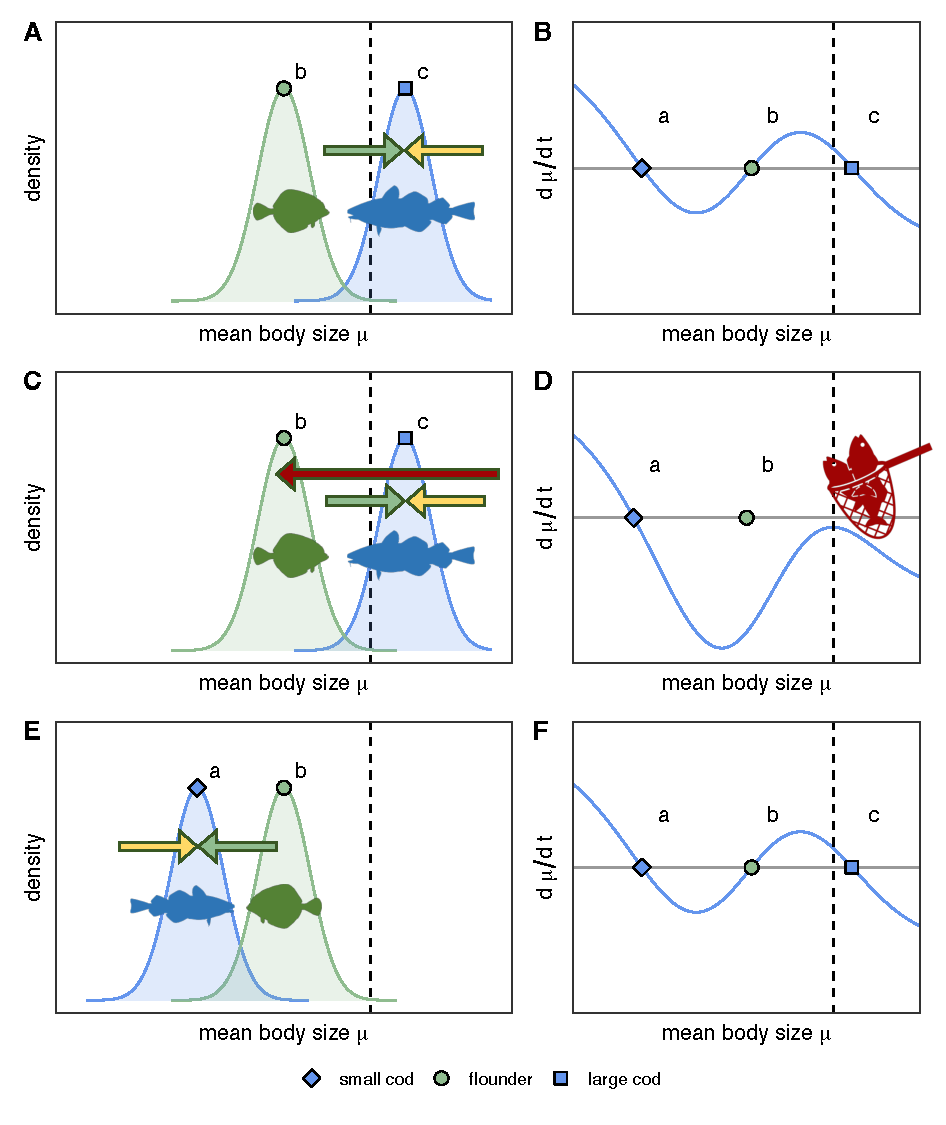
\includegraphics[width=1\linewidth]{fig1.pdf}
\caption{Conceptual figure of the model. Panels A,C,E: cod (blue) and flounder (green) relative body size distributions. Interspecific competition is assumed to increase as the difference between the body size distributions decreases. Arrows represent different sources of selection: green is the selective pressure from flounder competition, yellow from environmental effects, and red from fishing. The dashed lines show the cod's ``ideal'' body size which it would evolve to without competition and fishing. Panels B,D,F: Rate of change of cod mean body size as a function of cod mean body size. Positive (negative) values of $\text{d}\mu/dt$ increase (decrease) cod mean body size. For example in panel B, when mean body size is smaller than $a$, body size increases, while between points $a$ and $b$ body size decreases, making point $a$ a stable equilibrium. Correspondingly, point $c$ is an alternative stable state when cod body size starts larger than $b$. In panel D the rightmost two equilibria are absent (point $b$ is still shown for reference) due to the presence of active fishing which disproportionately selects large cod, overpowering the counterposing pressure from flounder competition.}
\label{fig:sizegrid}
\end{figure}

%As long as the mean cod body size remains larger than the unstable equilibrium, competition will keep the cod body size at its larger state---to some extent, even when adding an external selective pressure such as fishing. However, strong enough fishing pressure (Fig.~\ref{fig:sizegrid}D) will overcome the competitive pressure, forcing cod body size to go below the flounder body size and cross into the alternative smaller-sized stable state. 

%Subsequently, even after removing fishing and thus restoring the rate of change function in cod body size to that of Fig.~\ref{fig:sizegrid}F, cod size will be locked into the smaller body size equilibrium. The competitive pressure from flounder will now keep the cod away from energy-efficient prey, hindering cod from growing larger even though the ideal body size for the cod is set to $z^{*} = 1$.

\subsection*{Empirical evidence}

We use empirical data from cod and flouder populations in the Baltc Sea to evaluate our model. Different areas of the Baltic Sea have different relative proportions of cod and flounder. Subdivisions 25 and 28 (Fig.~\ref{fig:biomass_diet}A) are two examples of areas where cod is more abundant than flounder (subdivision 25) and vice versa (subdivision 28). In an area with a larger proportion of flounder, they will likely exert higher competitive pressure on the cod population via the elevated flounder densities $F$ (Eq.~\ref{eq:m_cod_r_z}, assuming constant resource densities over time). This will force the cod to evolve a larger dietary distance from the flounder, finding the best compromise between keeping a good dietary distance from the flounder while still having access to its preferred food items. Hence, we'd expect the diets of the two species to be less similar than in areas with a smaller proportion of flounder. Indeed, we observe a larger dietary difference between cod and flounder in subdivision 28, with proportionally less cod, than in subdivision 25 (Fig.~\ref{fig:biomass_diet}B).

\begin{figure}%[tbhp]
\centering
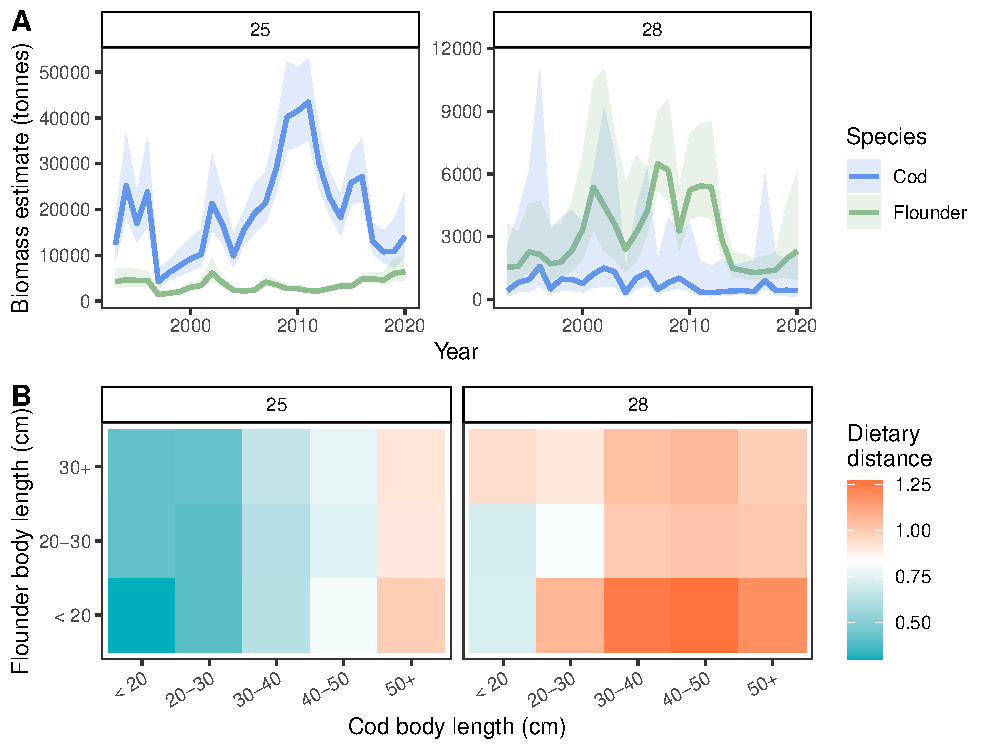
\includegraphics[width=1\linewidth]{fig3.pdf}
\caption{A: biomass model estimates of cod and flounder in subdivisions 25 and 28 in the Baltic Sea for years 1993-2020, with shaded areas representing the 95\% confidence interval (note the different scales on the y-axes). B: Spearman dietary distance based on stomach content of cod and flounder for different size classes in the two subdivisions, where a distance of 0 would indicate perfectly correlated diets. Here the data have been aggregated over years 2016-2020.}
\label{fig:biomass_diet}
\end{figure}

Body sizes of cod in both subdivisions have decreased over time, losing the largest individuals while smaller individuals have become more prevalent (Fig.~\ref{fig:sizedist}). This change occurred to a larger extent in subdivision 28 than in 25 in the period 1993--2020, with average cod lengths having decreased by 10.2 cm and 21.2 cm for subdivisions 25 and 28, respectively. Meanwhile, diets differ more between cod and flounder in subdivision 28 than in subdivision 25 (Fig.~\ref{fig:biomass_diet}B). Small-sized cod generally have a more similar diet to flounder, but that trend is less clear in subdivision 28, where the biggest drop in body size has occurred. The larger differences in diet in subdivision 28 are partly explained by smaller cod swapping benthic prey for a more piscivorous diet, thus diverging more from the benthic-specialized flounder (Supplementary Fig.~\ref{fig:si_prop_fish}).

\begin{figure}%[tbhp]
\centering
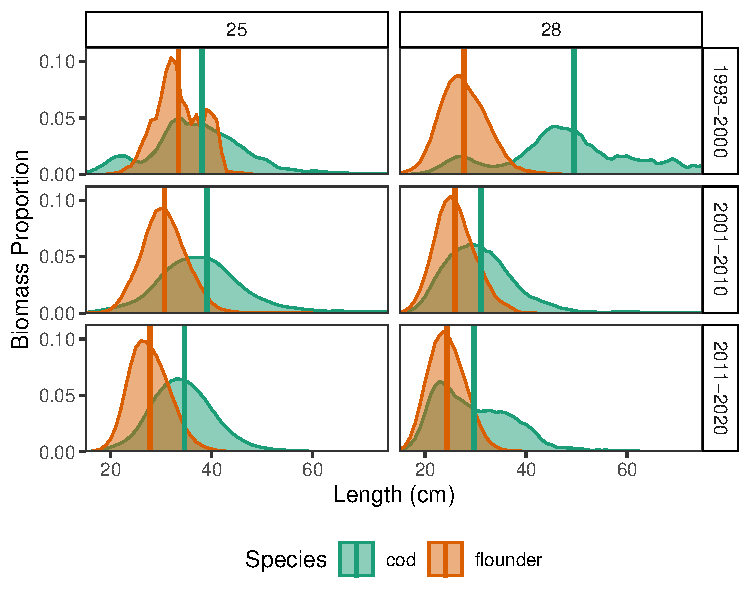
\includegraphics[width=1\linewidth]{fig4.pdf}
\caption{Cod and flounder length distributions in subdivisions 25 and 28 (facet columns) in the Baltic Sea. Data are aggregated across years listed in the facet rows for quarter 4 data. Vertical lines indicate mean length. Visual x-axis cutoff at 75 cm. Proportion is derived from biomass density for the specific lengths using 3 cm moving averages. For quarter 1 data see Supplementary Fig.~\ref{fig:si_sizegrid_q1}.}
\label{fig:sizedist}
\end{figure}

\section*{Discussion}

In this work, we investigated one possible reason why collapsed populations are unable to recover, even after alleviating the external pressure initially causing the collaps. We focus on how species interactions (e.g. competition) can play a key-role for locking ecosystems into different, potentially less preferrable, stable states. We examplify this with the highly actual problem of the collapsed cod population in the Batic Sea. The hypothesis is that cod have changed to such small sizes in response to intense fishing and that competition from flounder now prevents them from growing in body size again even when fishing pressure is considerably decreased. The combination of the diminished body size and increased competition has led to a change in the cod's diet, locking the cod in an alternative stable state. Using an eco-evolutionary model, we demonstrated that this is a feasible outcome under a set of plausible assumptions. Long-term survey data on cod and flounder stocks from the Baltic Sea support this hypothesis.

Cod diet differs strongly between size classes, whereas flounder have a quite narrow diet, and undergo only a limited allometric dietary shift \citep{Haase2020}. As such, smaller-sized cod compete for food with flounder of all size classes. When external pressures give smaller cod individuals an advantage over larger individuals, ultimately causing a genetic shift in the cod's size distribution, the flounder exerts a strong competitive pressure on the entire cod population. The interspecific competition acts as an effective ecological force for keeping cod locked into smaller sizes. Subsequently, even if the external pressure weakens, it will not necessarily be enough for the cod to recover to the state with larger body size. Our model effectively demonstrates the plausibility of this mechanism by identifying the equilibrium for cod body size when cod experience competition with flounder and different levels of fishing pressures: as long as cod has a mean body size large enough compared to flounder, competition will keep the cod at that large body size. However, when fishing pressure is intense enough and selectively targeting larger individuals, this will force cod body size to a small enough size that it loses its competitive advantage to flounder. The only stable equilibrium for cod is now the smaller size one, and even if fishing pressure is removed cod size will be locked into that equilibrium by the competitive pressure from flounder. Hence, the unstable equilibrium related to the flounder body size will act as a tipping point that the cod must overcome to change between the two alternative states of small and large cod \citep{Dakos2022}.

But how can we know that competition between the two fish species has been strong enough and affected their ecological niches? One option is to look at how their diets and local abundances have changed over time. In several areas of the Baltic Sea, dietary shifts have been observed in the cod populations \citep[e.g.][]{Kulatska2019, Haase2020, Neuenfeldt2020}, where smaller-sized cod have shifted from primarily feeding on benthic invertebrates towards a more piscivorous diet. However, historically, smaller cod have adhered to benthic diet more similar to flounder diet. The shift towards a more piscivorous diet applies in particular to areas with larger flounder populations (Supp. Fig.~\ref{fig:si_prop_fish}, subdivision 28). The survey data we analyzed here shows that in an area with more flounder than cod, the latter is on average smaller and overlaps less in their diet with flounder. This pattern could suggest that when cod body size has been reduced to a large extent due to external selective pressure (e.g., fishing, hypoxia), increased competition from flounder may keep cod away from the more favourable benthic diet \citep{ICES2015} and as such preventing population re-growth. 

That interspecific competition for food can play an important role when collapsed cod populations fail to recover, has been suggested by several studies. For example, \citep{Bundy2005} showed how small cod of the eastern Scotian Shelf stock appeared, after its collapse in 1993, to face a higher than average level of competition for resources. \citep{Walters2001} suggested that the lack of "cultivation effects", where large-sized adults suppress fishes that are predators or competitors of their juveniles, may be an important factor when populations depleted by fishing fail to recover.

In addition, other external factors can synergize with the interspecific competition further strengthening the negative effects. For example, including hypoxia in our model's current design does not provide any new dynamics, but instead reinforces the same effect that fishing exerts. Hypoxia is thought to affect larger individuals more negatively than smaller ones. In the Baltic Sea cod, there is a trend of larger cod dwelling in  low-oxygen waters, thus further reducing their condition \citep{Casini2021, Lindmark2023}. The higher metabolic needs of larger individuals may be a driver for their behaviour of utilizing hypoxic areas while foraging \citep{Reale2010}.

Our model shows that a cod population with smaller body size can recover after removed selection from fishing and reduced competition from flounder. However, if the shift in body size has indeed also resulted in a genetic shift, the speed of this recovery may be very slow, depending on how strong the selection towards larger body sizes is \citep{Ahti2020}. Larger body size is generally positively influenced by natural selection, as e.g. survival from natural predation is often improved with larger body size \citep{Olsen2011}. Further, regarding reproductive output, cod follow a hyper-allometric scaling where larger individuals can produce much more offspring than multiple smaller individuals of the same total weight \citep{Barneche2018}. This would further contribute to a natural selection towards bigger individuals if not restricted by other factors. Thus, the negative effects for a population depleted by large individuals will have far-reaching effects on recruitment and population recovery.

One could argue that the shift in body size distribution towards smaller individuals is due to selective fishing has removed all old and large individuals, rather than that a phenotypic change has occurred. However, in recent years the Baltic cod has become mature at smaller sizes \citep{Koster2017} which indicates that a genetic shift is plausible, and as such the empirical data support our model. Nevertheless, to further strengthen our reasoning, longer time series regarding both cod and flounder abundances and diet data for flounder over the time span when the cod population was thriving would be desirable. 

There are definite limitations to our modeling approach, and how we connect its results back to reality using our empirical data. First, we model one single trait when in fact several traits will be affected simultaneously and those traits may not evolve in the same direction and with the same speed. For instance, fishing likely selects for both growth and body size but potentially in different ways, because growth is the net result of multiple processes \citep{Rubalcaba2020}. As such, while body size is both directly targeted by fishing and is important for the presence or absence of species interactions, in particular in aquatic environments \citep{Ings2009}, we model a much-simplified scenario. Second, we assume that what we see in the dietary data of cod and flounder are effects of competitive interactions that already have taken place and that we now look at a new steady-state of the system. We also assume that those dietary shifts in cod depended on, at least to a large extent, competition from flounder, while they could in theory also be due to changes in prey availability via e.g., changes in spatial overlap or abundance of prey \citep{Enberg2012}.  We have not included factors such as potential changes in the community of prey species and the potential spatial effects on cod size and prey abundance. Lastly, while the model can produce the demonstrated bistability under a wide range of circumstances, its empirical interpretation critically depends on the fact that in the absence of both fishing pressure and competition from flounder, cod would evolve to occupy the flounder's size niche. Otherwise, cod would evolve towards larger body sizes in Fig.~\ref{fig:sizegrid}AC even without the influence of the flounder. Therefore, the observed pattern that the more flounder correlates with a larger dietary distance would lose its connection with competition and would be explained by other mechanisms that are not considered by our model at all.

\subsection*{Conclusions}

Fishing directly selects against a large body size in the fished populations, and can therefore cause evolution toward smaller body sizes in the targeted species. Body size is tightly coupled to species-specific factors, but also many ecological features, such as competitive and trophic interactions. Interspecific interactions are strong forces in shaping ecological communities, and body downsizing can therefore reshape natural selection and via eco-evolutionary feedback loops act back on body size of the harvested species \citep{Edeline2021}. Our eco-evolutionary model pinpoints the mechanisms behind the synergistic effects of external pressures and species competitive interactions on body size and highlights the importance of taking evolutionary changes into account for achieving successful ecosystem management in the Baltic Sea and elsewhere.

\matmethods{

Our eco-evolutionary model assumes that (1) there is variation in some heritable trait $z$, (2) this trait determines diet, and (3) competition increases with more similar diets. The trait $z$ is identified with body size, but only in a relative, prey-determining sense \citep{Schneider2016}. That is, we assume that the body size of cod and the average size of its prey are sufficiently tightly correlated that $z$ need not refer to the actual cod body size, but instead to the mean body size of its prey. The advantage of this is to simplify our use of language: now we can say ``cod and flounder of equal size'' instead of saying ``a size difference between cod and flounder such that their prey are of equal average size''. Thus, we define $z = \log(B/B_0)$, where $B$ is the average prey size (assumed to be in an essentially one-to-one relationship with the cod or flounder individual's size) and $B_0$ is a reference size which can be chosen without loss of generality. Here we set it to be the mean size $\mu_F$ of the flounder's prey. This choice means that $z = 0$ now corresponds to the point at which the mean prey size of cod and flounder coincide: $z = \log(\mu_F/B_0) = \log(B_0 / B_0) = 0$. To simplify the model, we keep the flounder body size distribution fixed while it exerts competitive pressure on cod to reduce trait similarity, and thus diet overlap. From this assumption, it also follows that $B_0$ is a fixed constant in the model.

The cod also have other, intrinsic limits to how large they can grow, e.g.\ from increased metabolic demands and other physiological growth-limiting mechanisms \citep{Metcalfe2003}. These two opposing selective pressures create an equilibrium for the cod size at point $c$ in Fig.~\ref{fig:sizegrid}A. Then there is fishing (Fig.~\ref{fig:sizegrid}CD) which actively selects large cod individuals, forcing the population towards smaller sizes. If selection from fishing is stronger than the competitive pressure from flounder, the cod can be pushed into an alternative stable state with diminished body size (Fig.~\ref{fig:sizegrid}D, point $a$). Now, with the cod size distribution in panel E, the flounder competitive effect is inverted, which keeps the cod locked in its smaller state even when relieving the fishing pressure (Fig.~\ref{fig:sizegrid}F, point $a$). 

The per capita growth rate of cod individuals with size $z$ depends on a size-dependent intrinsic rate $r_{0}(z)$, a size-dependent fishing pressure $f(z)$, a size-dependent effect of oxygen-deprived regions $H(z)$ (which affects bigger individuals more due to different food-seeking behaviour), and competition from individuals with size $z'$, denoted $a(z,z')$. The competition term includes both intraspecific competition with other cod and interspecific competition with flounder. The per capita growth rate of cod with size $z$ is therefore given by
\begin{equation}
  \label{eq:m_cod_r_z}
  r(z) = r_{0}(z) - f(z) - H(z) - N\int a(z,z') p(z') \,\ud z' - F\int a(z,z') p_F(z') \,\ud z',
\end{equation}
where $N$ and $p(z)$ are the cod population density and size distribution, respectively; similarly, $F$ and $p_F(z)$ are the flounder population density and trait distribution. These appear under integrals, because the contribution to competition from all traits $z'$ are added up to obtain the total competition experienced by cod, both from itself and from the flounder.

Given the assumption that body size variation is determined by a multitude of additive loci where each locus has a small effect on body size, the infinitesimal model of quantitative genetics \citep{Barton2017} is suitable to model the eco-evolutionary dynamics for the growth rates
\begin{equation}
\label{eq:m_N}
    \frac{\text{d}N}{\text{d}t} = N \int r(z) p(z) \text{d}z ,
\end{equation}
\begin{equation}
\label{eq:m_mu}
    \frac{\text{d}\mu}{\text{d}t} = h^{2} \int (z-\mu)r(z)p(z)\text{d}z,
\end{equation}
where $\mu$ is the mean of the cod size distribution $p(z)$, and $h^{2}$ is the trait's heritability \citep{Barabas2016, Pastore2021}. Another consequence of the quantitative genetic limit is that the size distributions for cod $p(z)$ and flounder $p_{F}(z')$ follow normal distributions (Eqs.~\ref{eq:normdist-cod} and \ref{eq:normdist-flounder}). Note that this means treating every individual as having one particular size; in other words, we are ignoring ontological niche shifts that are important for determining diet \citep{WernerGilliam1984}. This is definitely a shortcoming of the model, but one that likely only affects the quantitative details more than the basic mechanism that is our focus here.

For the intrinsic growth rate of cod, $r_{0}(z)$, we assume that growth is restricted to a limited size range, where too big or too small size constrains growth due to lack of prey or physiological limits according to
\begin{equation}
  \label{eq:m_r0}
  r_{0}(z) = \varrho \left( 1- \frac{(z-z^*)^2}{\theta^{2}} \right).
\end{equation}
Here $\varrho$ scales the maximum of the growth curve, while $\theta$ determines the width of the size range in which growth is possible. The optimal size for cod growth is $z^{*}$.

Both the fishing function $f(z)$ (Eq. \ref{eq:fishing}) and the hypoxic effect function $H(z)$ (Eq. \ref{eq:hypoxia}) are sigmoid responses, with smaller effects on smaller individuals and larger effects on larger individuals. Finally, the competition kernel $a(z,z')$ is given by a Gaussian form that declines with increasing trait difference:
\begin{equation}
    \label{eq:m_compkern}
    a(z,z') = \alpha_0 \exp\left(-\frac{(z-z')^2}{\omega^{2}} \right) ,
\end{equation}
where $\alpha_0$ is the maximum interaction strength, and $\omega$ describes the difference in body size needed to reduce the effect of competition. By substituting these components into Eqs. \ref{eq:m_N} and \ref{eq:m_mu}, we obtained the full model describing the eco-evolutionary dynamics of the cod (Supplement \ref{sec:si_ecoevo}). 


\subsection*{Survey data}

We relate the mechanisms of our eco-evolutionary model to cod and flounder populations in the Baltic Sea. Using available survey data for both species, we compare model expectations with observed biological data to support the model's conclusions. 

We used data from the Baltic International Trawl Survey (BITS) to evaluate relative biomasses and diets of cod and flounder in the southern Baltic Sea. BITS is a bi-annual bottom trawl survey, conducted during quarters one and four. Data on catch per unit effort can be downloaded from the ICES DATRAS database (\texttt{https://datras.ices.dk/}). We standardized these data for differences in gear following \citep{Orio2017, Lindmark2023}, to acquire survey catches in density per area (kg/km\textsuperscript{2}). We fit these data with a geostatistical generalized linear mixed-effects model, using a Tweedie distribution \citep{Tweedie1984, Shono2008, andersonSdmTMBPackageFast2022} and a log-link function, due to the presence of zeros and continuous densities. 

For details about the biomass model, we refer to Supplement \ref{sec:si_biomass} and \citep{Lindmark2023}. We used this model to predict the biomass density of cod and flounder over a regular grid of 4 $\times$ 4 km squares with covariates to calculate indices of relative biomass based on a random-field model \citep{Shelton2014, Thorson2015} over the spatial domain. While the model was fit to data from years 1993–2020 in ICES subdivisions 24-28, we only make predictions for subdivisions 25 and 28 to match where we have the most diet data (Supplementary Fig.~\ref{fig:si_map}). Cod and flounder size distributions were also extracted from the DATRAS database. Distributions are shown as proportion of biomass per length class, where each length is a 3 cm moving average (Quarter 4 data Fig. \ref{fig:sizegrid}, quarter 1 data Fig. \ref{fig:si_sizegrid_q1}). Years were aggregated with a finer span for the earlier years when the biggest turnover in distributions occurred.

Cod and flounder stomach contents were collected during the BITS survey by the Swedish University of Agricultural Sciences, Department of Aquatic Resources, following the BITS protocol (ICES 2017). The stomach samples included data for individuals larger than 6 cm, and we used only data from the survey conducted in quarter one because of the higher number of trawl hauls and stomach samples. Whenever possible, one flounder and one cod stomach were collected for each cm class of fish length and trawl haul. 

We used the stomach content data to calculate the dietary distance between cod and flounder. The dietary distance was used to estimate interspecific competition for the same prey items. Dietary distances were calculated separately for each subdivision, and were based on the number of prey items on a species level. We aggregated cod and flounder data into arbitrary length classes (Cod $<$ 20 cm, 20-30 cm, 30-40 cm and $>$ 50 cm, flounder $<$ 20 cm, 20-30 cm, and $>$ 30 cm). For calculating the distances, the Spearman method was used.
}

\showmatmethods{} % Display the Materials and Methods section

\acknow{Åke Brännström for valuable feedback on the manuscript.}

\showacknow{} % Display the acknowledgments section


\bibsplit[23]
%Use \bibsplit to split the references from the body of the text. Value "[2]" represents the number of reference in the left column (Note: Please avoid single column figures & tables on this page.)

% Bibliography
\bibliography{references}

\end{document}
